% Chapter 3

\chapter{Methodology} % Write in your own chapter title
\label{Chapter3}
\lhead{Chapter 3. \emph{Approach of Weather Classification}}

\section{Dataset}

There are over 15 million labeled images in ImageNet database belonging to about 22,000 categories. The images were collected from the Internet and labeled manually. From 2010, an annual competition named the ImageNet Large-Scale Visual REcognition Challenge (ILSVRC) has been held. The competition uses a subset of dataset which is 1000 images in 1000 categories. Totally, there are over 1 million training images and 50,000 validation images and 150,000 images for testing.
\graphicspath{ {./Figures/} }
\begin{figure}[!htb]
    \centering
	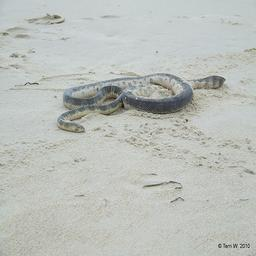
\includegraphics[width=0.4\textwidth]{ILSVRC2012_val_00000001.JPEG}
    \qquad
    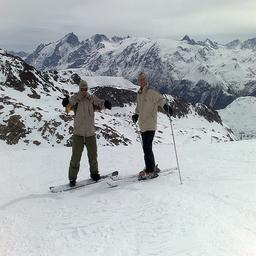
\includegraphics[width=0.4\textwidth]{ILSVRC2012_val_00000002.JPEG}
    \caption{2 Figures from ImageNet}%
    \label{fig:ImageNetExamples}%
\end{figure}

For weather dataset, it contains 10,000 images for two categories evenly, cloudy and sunny. They are from three sources, Sun Dataset\citep{russell2008labelme}, Labelme Dataset\citep{xiao2010sun} and Flickr. They were classified manually and similar images are removed. There are no unambiguous images.
\graphicspath{ {./Figures/} }
\begin{figure}[!htb]
    \centering
	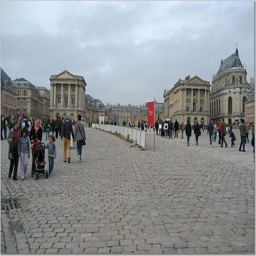
\includegraphics[width=0.4\textwidth]{cloudy_0001.png}
    \qquad
    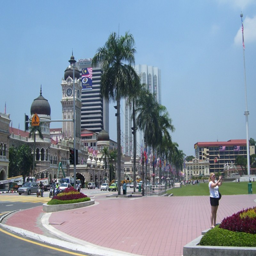
\includegraphics[width=0.4\textwidth]{sunny_0003.png}
    \caption{2 Figures from Weather Dataset}%
    \label{fig:WeatherExamples}%
\end{figure}

The two datasets are different. ImageNet dataset is for object classification and weather dataset is for scenes classification. Because the two datasets consists of different resolution images, we have to resize them to a fixed resolution of $256\times256$ for constant dimension input for neural networks. To train the model with ImageNet images, we resize shorter side of images to length 256 and then cropped out a $256\times256$ image from center.

\section{Data Argument}

\graphicspath{ {./Figures/} }
\begin{figure}[!htb]
    \centering
    \subfigure[original image]{
		\begin{minipage}{0.3\textwidth}
		   		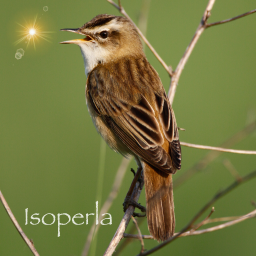
\includegraphics[width=1\textwidth]{crop}
		   		\label{fig:orig}
		\end{minipage}
    	} 
    \subfigure[cropped from left up]{
		\begin{minipage}{0.3\textwidth}
		   		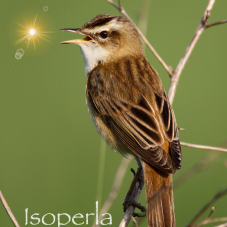
\includegraphics[width=1\textwidth]{cropleftup}
		   		\label{fig:leftup}
		\end{minipage}
    	} 
    \subfigure[cropped from left down]{
		\begin{minipage}{0.3\textwidth}
		   		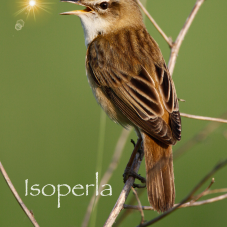
\includegraphics[width=1\textwidth]{cropleftdown}
		   		\label{fig:leftdown}
		\end{minipage}
    	} 
    \subfigure[cropped from right up]{
		\begin{minipage}{0.3\textwidth}
		   		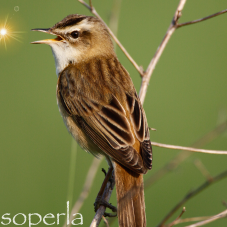
\includegraphics[width=1\textwidth]{croprightup}
		   		\label{fig:rightup}
		\end{minipage}
    	} 
    \subfigure[cropped from right down]{
		\begin{minipage}{0.3\textwidth}
		   		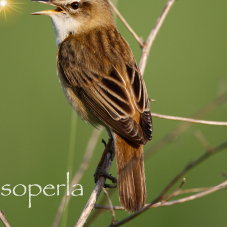
\includegraphics[width=1\textwidth]{croprightdown}
		   		\label{fig:rightdown}
		\end{minipage}
    	} 
    \subfigure[cropped from center]{
		\begin{minipage}{0.3\textwidth}
		   		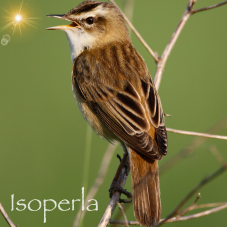
\includegraphics[width=1\textwidth]{cropcen}
		   		\label{fig:cropcen}
		\end{minipage}
    	} 

    \caption{A set of cropped patches from original image}%

    \label{fig:dataargument}%
\end{figure}
The model has about 60 million neurons, and it is essential to avoid overfitting. One of methods is to do data argument. Dataset is artificially enlarged via image transformations and horizontal reflections. For each $256\times256$ image, the network extracts five $224\times224$ patches from four corners and center and reflects them horizontally. Hence, there are 10 patches for 1 image in total. Figures \ref{fig:dataargument} show the method of data argument.
% add image examples here

\section{Spatial Pyramid Pooling}

The factors which have effects on scene classification can be any spatial positions in the image. Spatial pyramid pooling can help to solve the problem.

A spatial pyramid pooling layer is deployed behind the fifth convolutional layer. A set of bin sizes are set to discern different size local information from output of the fifth convolutional layer.  A sliding window pooling  is implemented on the feature maps after the fifth convolutional layer. Assuming dimension of feature map is $axa$ and bin size is $n$, each window size is $\lceil a/n \rceil$ and stride size is $\lfloor a/n \rfloor$ where $\lceil \rceil$ and $\lfloor \rfloor$ denote ceiling and flooring operations. For $l$ level pyramid, there are $l$ spatial pyramid pooling layers, The the $l$ layers will be concatenated into a fully connected layer. The bin sizes are 1, 2, 3 and 6.

\begin{figure}[htb]
    \centering
	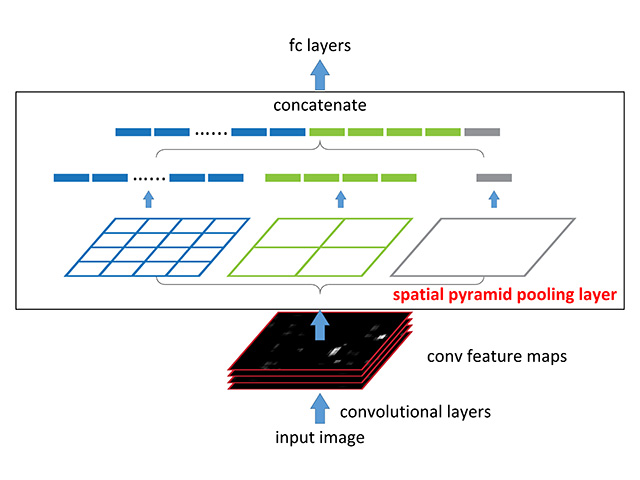
\includegraphics[width=0.8\textwidth]{sppnet.jpg}
    \caption{Diagram of Spatial Pyramid Pooling layer}%
    \label{fig:sppnet}%
\end{figure}

With implementing spatial pyramid pooling layers in convolutional neural networks, all contribution of different scales are considered.

\section{Convolutional Neural Networks Architecture}

Due to the significant performance of AlexNet \citep{krizhevsky2012imagenet} deep convolutional neural networks, we train a model based on it. The architecture of the network has seven hidden adaptive layers-five convolutional and two fully connected layers.
\begin{figure}[htb]
    \centering
	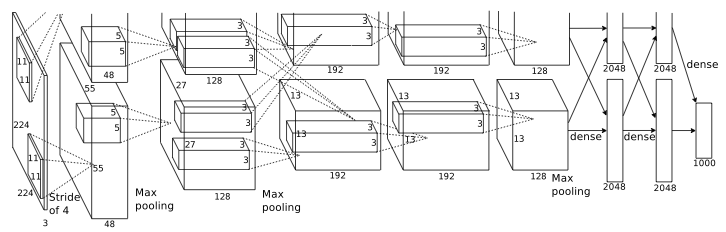
\includegraphics[width=0.8\textwidth]{AlexNet.png}
    \caption{Architecture of AlexNet}%
    \label{fig:ImageNetArch}%
\end{figure}
The network is very deep and the early layers are split over on two GPUs. It is able to give $62.5\%$ accuracy rates with one prediction and $83\%$ accuracy rates with five predictions.

The network replaces each neuron's outputs nonlinearity function $f$ from $f(x) = tanh(x)$ or $f(x) = (1 + e^{-x})^(-1)$ to Rectified Linear Units(RELUs)\citep{nair2010rectified} which can accelerate learning speed several times faster than $tanh$ function. 

In the network, there are three types of layers and they play different roles in the model. The input data dimension is $224\times224\times3$ which means the raw pixel value stored in a width 224, height 224 and with three color channels R,G,B matrix. In the first convolutional layer, there are 98 kernel of size $11\times11\times3$ with stride size 4 and outputs are 96 neurons. A max pooling layer downsamples the spatial dimensions. The second convolutional layer filters output of previous pooling layer with kernel size $5\times5\times48$. The third convolutiona layer owns 384 kernels of $3\times3\times256$ and receives outputs of the second convolutional layer. The fourth convolutional layer has 384 kernels of size $3\times3\times192$ and the last convolutional layer has 256 kernels of size $3\times3\times192$. Each fully connected layers have 4096 units. At the end of network, there is a softmax layer with 1000 outputs.
\begin{table}[h]
\begin{center}
    \begin{tabular}{ | c | p{8cm} | }
    \hline
    Layer Name & Layer Description \\ \hline
    Input & 224 $\times$ 224 RGB image \\ \hline
    CONV1 & 11 $\times$ 11 conv, 96 ReLU units, stride 4 \\ \hline
    POOL1 & 3 $\times$ 3 max pooling, stride 2 \\ \hline
    CONV2 & 5 $\times$ 5 conv 256 ReLU units, stride 1 \\ \hline
    POOL2 & 3 $\times$ 3 max pooling, stride 2 \\ \hline
    CONV3 & 3 $\times$ 3 conv 384 ReLU units, stride 1 \\ \hline
    CONV4 & 3 $\times$ 3 conv 384 ReLU units, stride 1 \\ \hline
    CONV5 & 3 $\times$ 3 conv 256 ReLU units, stride 1 \\ \hline
    POOL5 & 3 $\times$ 3 max pooling, stride 2 \\ \hline
    SPP & bin size 1,2,3,6 \\ \hline
    FC6 & fully connect, ReLU 4096 units\\ \hline
    FC7 & fully connect, ReLU 4096 units\\ \hline
    FC8 & fully connect, ReLU 1000 units\\ \hline
    SOFTMAX & 1000 way softmax\\ \hline
    \end{tabular}
    \caption{Parameters of model}
    \label{fig:NetPara}
\end{center}
\end{table}

















